%======================================================================
\chapter{Measuring R\'{e}nyi Entanglement Entropy}
%======================================================================
\section{The Swap Operator}

\begin{figure} {
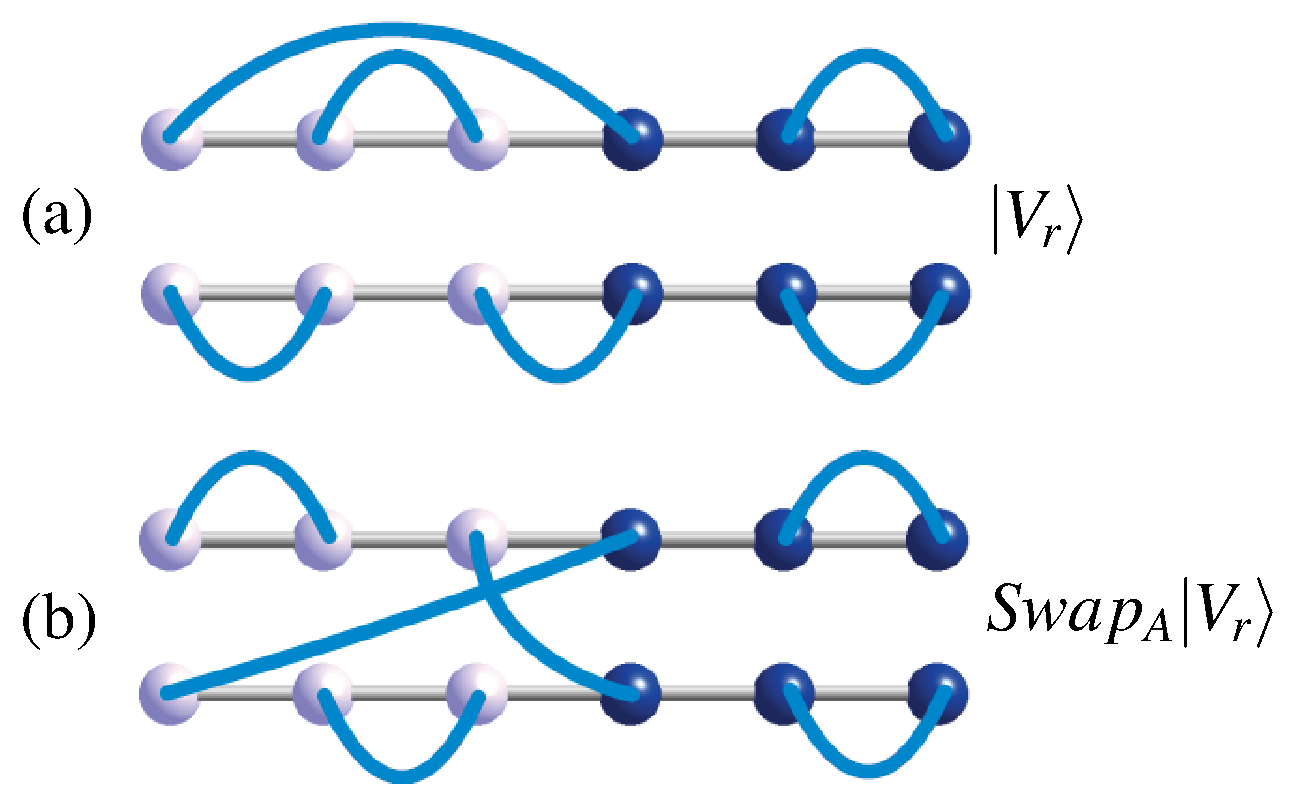
\includegraphics[width=6.5 in]{./figures/paper2/fig_swap/swap_2.eps} 
\caption[Swap operator]{
\label{swap_2}
{\color{red}
A six-site chain, with two non-interacting copies (top and bottom) before
(a) and after (b) the $Swap_A$ operation. % in the valence bond basis.  
The region $A$ consists of three light-colored sites on the left; the
complement region $B$ of three dark sites on the right.  The curved lines denote
singlets in the state $|V_{r}\rangle$, which is a product of two
different valence bond states, one per copy.
The ground state of the entire system is a linear combination of similar $|V_{r}\rangle$.
}
}
} \end{figure}


\section{1D Results}

\begin{figure} {
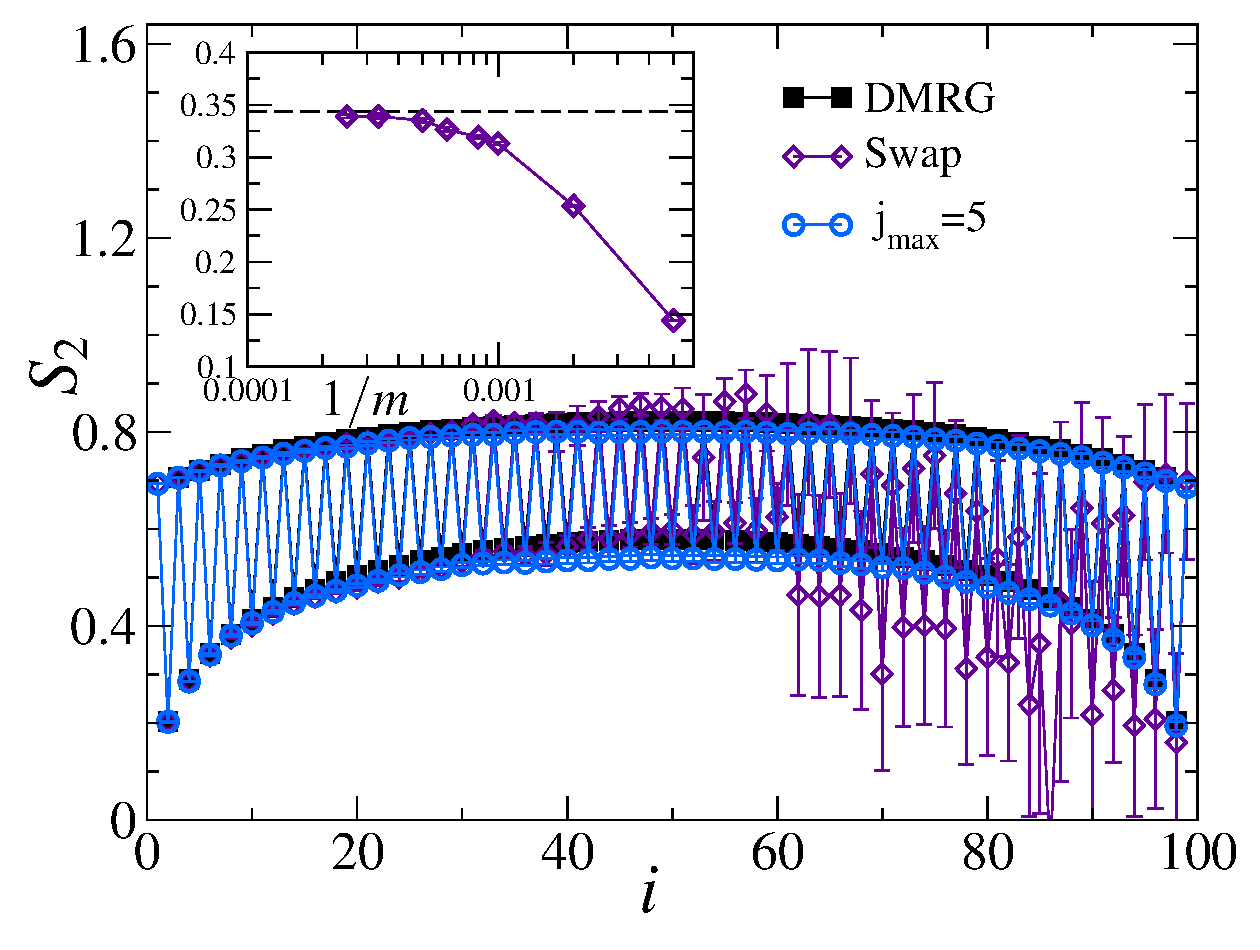
\includegraphics[width=6.2in]{./figures/paper2/fig_1D/L100_fig2.eps} 
\centering
\caption[Renyi for 100 site chain]{ 
\label{1Dfig}
{\color{red}
The Renyi entropy $S_2$ as a function of site index $i \in A$, for a 100-site Heisenberg chain with open boundaries, 
calculated with DMRG and QMC.  Data labeled ``Swap'' was calculated with Eq.~eqref{Swap} with one QMC simulation, while
data labeled $j_{\rm max}=5$ was calculated with Eq.~eqref{Ratio} using 20 separate QMC simulations with a range of  $j \in [1,5]$.  The inset shows the convergence of $S_2$ to the exact value (dashed line) for $i=6$ with up to $m=4000$.
}
}
} 

\end{figure}

\section{The Ratio Operator}

\section{2D Results}

\section{The Area Law}
